\experiment{Planteamiento Teórico}
Se desarrolla el fundamento teórico del problema de los tres péndulos
físicos acoplados por resortes. A partir del desplazamiento angular
de cada péndulo, \(\theta_i\), se establece el sistema planteado con
sus relaciones importantes, presentado en la \cref{fig:sistema-pendulos}.

\begin{figure}[htbp!]
  \centering
  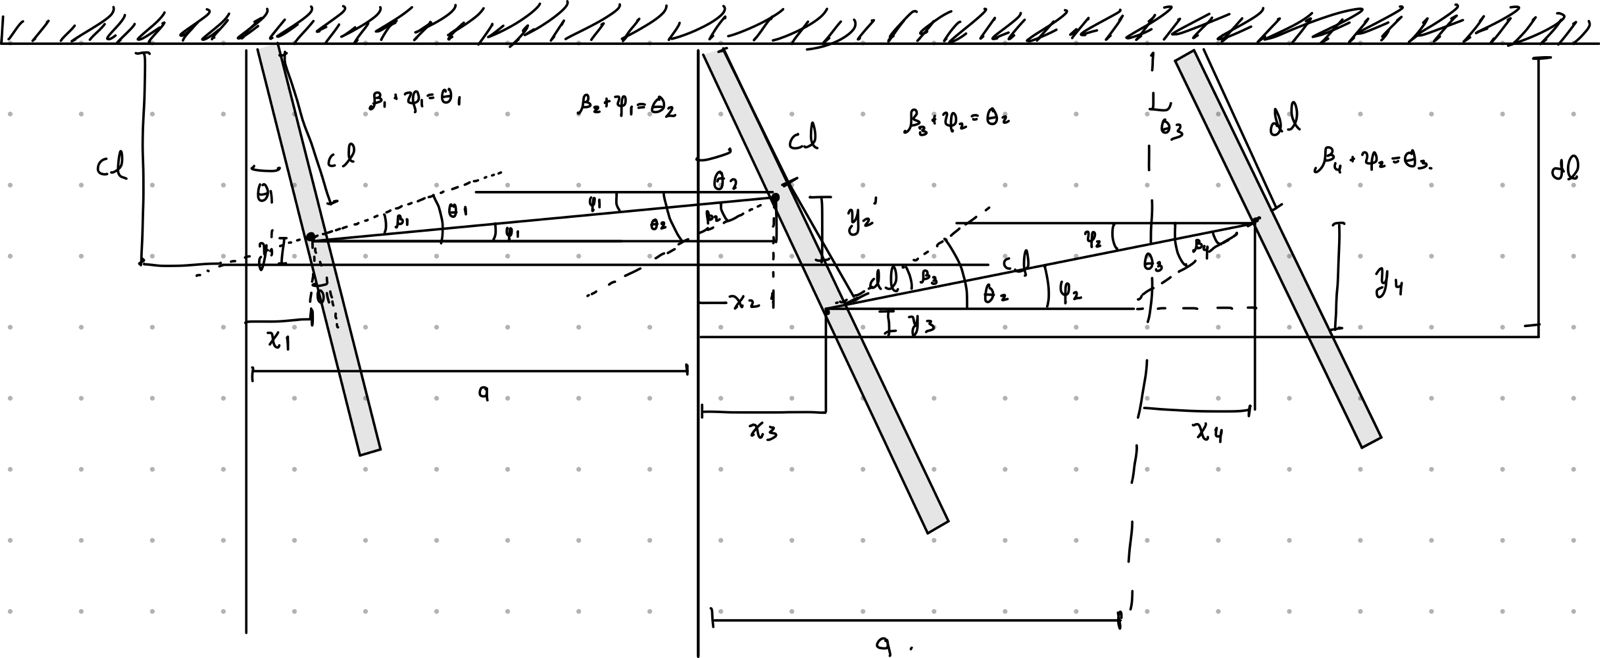
\includegraphics[width=0.8\linewidth]{Figures/IM1.jpeg}
  \caption{Sistema de tres péndulos físicos acoplados por resortes.}
  \label{fig:sistema-pendulos}
\end{figure}

Considerando el desplazamiento angular de cada péndulo, se determina
la suma de los torques que actúan sobre cada uno para derivar el
sistema de ecuaciones del movimiento.

La distancia \( a \) es la separación entre cada péndulo. \( cl \) es
la distancia a la cual se acoplan los péndulos 1 y 2 por medio del
resorte con constante \( k_1 \), mientras que \( dl \) es la distancia
de acople entre 2 y 3 por medio del resorte con constante \( k_2 \).
Los \(y_{\text{cm}_i}\) corresponden a la distancia desde el punto de
giro al centro de masa. De esta forma, el torque restaurador
gravitacional está relacionado con \(m_i g y_{\text{cm}_i} \sin{\theta_i}\).

Para las interacciones generadas por los resortes, se asume que
obedecen a la ley de Hooke lineal y que actúan a lo largo de una
línea de acción horizontal. De esta forma, se aplicará una
aproximación lineal a todos los términos angulares no lineales.

La sumatoria de torques para cada péndulo genera el siguiente
sistema de ecuaciones diferenciales:

\begin{equation}
  \begin{aligned}
    \ddot{\theta}_1 =\; &
    -\theta_1 \left[ \frac{k_1 (cl)^2 + y_{\text{cm}_1} m_1 g}{I_1} \right]
    + \theta_2 \left( \frac{k_1 (cl)^2}{I_1} \right) \\[0.5em]
    \ddot{\theta}_2 =\; &
    \theta_1 \left( \frac{k_1 (cl)^2}{I_2} \right)
    - \theta_2 \left[ \frac{k_1 (cl)^2 + k_2 (dl)^2 + y_{\text{cm}_2} m_2 g}{I_2} \right]
    + \theta_3 \left( \frac{k_2 (dl)^2}{I_2} \right) \\[0.5em]
    \ddot{\theta}_3 =\; &
    \theta_2 \left( \frac{k_2 (dl)^2}{I_3} \right)
    - \theta_3 \left[ \frac{k_2 (dl)^2 + y_{\text{cm}_3} m_3 g}{I_3} \right]
  \end{aligned}
\end{equation}

\experiment{Características Experimentales}
Adicionalmente, se establecen las características clave del montaje
experimental, buscando cumplir con las siguientes condiciones:

\begin{itemize}
  \item Usar barras masivas, de modo que, en comparación con
    constantes elásticas bajas de los resortes, se obtengan series
    de tiempo extensas. Esto es importante, ya que en el caso real
    se tiene rozamiento con el aire y en las zonas de contacto
    (rodamientos).
  \item Utilizar resortes que se aproximen al muelle ideal,
    manteniendo su linealidad y capacidad de operar bajo fuerzas
    compresivas y extensivas. Se buscarán constantes elásticas
    suficientemente pequeñas para permitir oscilaciones extensas y
    claras.
  \item Obtener barras ``ideales'', donde los puntos de contacto
    estén centrados y equidistantes en las tres barras.
\end{itemize}

Para lograr esto, se buscarán barras muy masivas, fabricadas con
un material de alta densidad, como un metal, descartando el aluminio
en primera aproximación debido a su baja densidad. Para la toma de
datos, se utilizarán sensores rotacionales angulares CASSY. Se
acoplará un sensor a cada péndulo/barra, aprovechando que cada sensor
está montado en un rodamiento que permite mayor libertad de
movimiento y cuenta con un soporte para colgar los objetos que rotan.

\begin{figure}[htbp!]
  \centering
  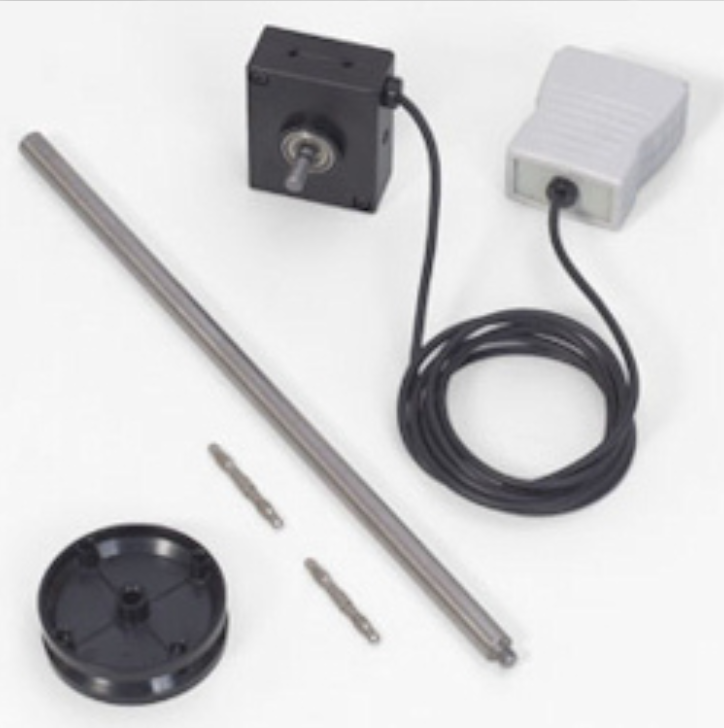
\includegraphics[width=0.5\linewidth]{Figures/IM2.png}
  \caption{Sensor CASSY de movimiento angular.}
  \label{fig:cassy}
\end{figure}
